% slides_full.tex -- integrated deck: ASM/sASM overlap anomaly -> attribution ->
% coarse-space construction -> cross-system (Sys1->Sys2->Sys3).
% compile: pdflatex slides_full.tex   (run in asm_bug_demo/dim_var/)
\documentclass[aspectratio=169,9pt]{beamer}
\usepackage[T1]{fontenc}
\usepackage{graphicx,amsmath,amssymb,booktabs,array,colortbl}
\usepackage{helvet}
\renewcommand{\familydefault}{\sfdefault}

\definecolor{navy}{HTML}{14233B}
\definecolor{teal}{HTML}{117A8B}
\definecolor{amber}{HTML}{C8841A}
\definecolor{asm}{HTML}{1F4E79}
\definecolor{sasm}{HTML}{C8641B}
\definecolor{muted}{HTML}{5B6B7B}
\definecolor{bg}{HTML}{F7F9FC}
\definecolor{cardln}{HTML}{DCE4EC}
\definecolor{good}{HTML}{1E7A46}

\setbeamercolor{normal text}{fg=navy}
\setbeamercolor{structure}{fg=teal}
\setbeamercolor{background canvas}{bg=bg}
\setbeamertemplate{navigation symbols}{}
\setbeamertemplate{itemize item}{\small\textcolor{teal}{\textbf{--}}}
\setbeamertemplate{itemize subitem}{\footnotesize\textcolor{muted}{\textbullet}}
\setbeamerfont{frametitle}{series=\bfseries}

\setbeamertemplate{frametitle}{%
  \vskip0.45em
  {\scriptsize\color{teal}\textbf{\MakeUppercase{\insertframesubtitle}}\par}\vskip0.05em
  {\large\color{navy}\bfseries\insertframetitle\par}\vskip0.1em}
\setbeamertemplate{footline}{%
  \hbox to\paperwidth{\hspace{0.6em}\tiny\color{muted}{ASM/sASM overlap $\to$ attribution $\to$ coarse $\to$ cross-system \textperiodcentered\ PETSc 3.24 / exact-spectrum lab}%
  \hfill\tiny\color{muted}{p.\,\insertframenumber}\hspace{0.6em}}\vskip2pt}

\newcommand{\rfig}[2][1.0]{\includegraphics[width=#1\linewidth,height=0.56\textheight,keepaspectratio]{results/#2}}
% spec line: bold teal label + text
\newcommand{\spec}[2]{\textcolor{teal}{\textbf{#1}}\,#2\par\smallskip}
\newcommand{\concl}[1]{\vfill\noindent\colorbox{navy}{\parbox{\dimexpr\textwidth-2\fboxsep\relax}{\color{white}\footnotesize\textbf{Conclusion.}\ #1}}}

\title{Overlapping Schwarz for the cardiac solver stack}
\author{Tianhao Ma}\date{2026-06}

\begin{document}

% ===================================================== 1 TITLE
{\setbeamercolor{background canvas}{bg=navy}
\begin{frame}[plain]
  \vspace{0.5em}{\color{teal}\rule{\linewidth}{2pt}}\par\vspace{1.0em}
  {\color{white}\LARGE\bfseries When does overlap help? Diagnosing and fixing\\[0.2em]
   ASM/sASM for the cardiac solver stack\par}\vspace{0.5em}
  {\color{white!80!teal}\large Overlap anomaly $\to$ spectral attribution $\to$ a non-GenEO coarse space $\to$ cross-system reuse (Sys1$\to$Sys2$\to$Sys3)\par}
  \vspace{1.0em}
  {\footnotesize\color{white}%
   \begin{tabular}{@{}p{0.3\linewidth}p{0.32\linewidth}p{0.3\linewidth}@{}}
   \textcolor{amber}{\textbf{Sys1}} monodomain\newline $(1/\Delta t)M+\theta K$, Neumann, easy &
   \textcolor{amber}{\textbf{Sys2}} $u_e$ recovery\newline pure-Neumann $K$, singular, hardest &
   \textcolor{amber}{\textbf{Sys3}} torso\newline different mesh, interface-Dirichlet \\
   \end{tabular}\par}
  \vspace{0.9em}{\small\color{white!70!navy}\texttt{CG + PCASM(ICC) + two-level} \textperiodcentered\ exact-spectrum NumPy lab + PETSc 3.24\par}
  \vspace{0.4em}{\color{amber}\rule{\linewidth}{2pt}}
\end{frame}}

% ===================================================== 2 ROADMAP
\begin{frame}{Roadmap}{overview}
  \begin{columns}[T]
  \begin{column}{0.62\linewidth}
  \begin{enumerate}\setlength\itemsep{0.45em}
   \item[\textcolor{amber}{\textbf{I}}] \textbf{The anomaly} — on SPD elliptic problems, unscaled BASIC ASM + inexact ICC + CG makes CG iterations \emph{rise} with overlap (cases a–d, unstructured P1 FEM).
   \item[\textcolor{amber}{\textbf{II}}] \textbf{Attribution} — which factor (dimension / boundary / shift) makes it hard, and through which spectral channel.
   \item[\textcolor{amber}{\textbf{III}}] \textbf{The fix} — a non-GenEO two-level coarse: shift-invariant $(K,M)$ spectral modes + known-coefficient A-harmonic modes.
   \item[\textcolor{amber}{\textbf{IV}}] \textbf{Cross-system} — one build-once coarse reused across Sys1$\to$Sys2 (same mesh) and Sys3 (different mesh).
  \end{enumerate}
  \end{column}
  \begin{column}{0.37\linewidth}\footnotesize
   \textcolor{teal}{\textbf{The unifying lens (all parts):}}\\[3pt]
   $\displaystyle\text{iters}\approx\tfrac12\sqrt{\kappa}\,\ln\tfrac2\varepsilon,\quad \kappa=\frac{\lambda_{\max}}{\lambda_{\min}}$\\[5pt]
   $\lambda_{\max}(\text{ASM})\approx\omega\cdot\hat N$\\
   $\lambda_{\max}(\text{sASM})\approx\omega$\\
   $\lambda_{\min}\sim 1/C_0^2,\ \ C_0^2\sim(1{+}H/\delta)$\\[5pt]
   \textcolor{muted}{$\hat N$=over-count (geometry), $\omega$=inexact-ICC, $\lambda_{\min}$=info transfer / coarse mode.}
  \end{column}
  \end{columns}
\end{frame}

% ===================================================== 3 MECHANISM
\begin{frame}{The mechanism: two spectral channels}{lens}
  \begin{columns}[T]
  \begin{column}{0.52\linewidth}\footnotesize
   \spec{ASM (BASIC):}{$M^{-1}=\sum_i R_i^\top A_i^{-1}R_i$ — overlap region added repeatedly $\Rightarrow$ over-count $\hat N=m_{\text{axis}}^d$.}
   \spec{sASM (weighted):}{$M^{-1}=D^{-1/2}(\sum_i R_i^\top A_i^{-1}R_i)D^{-1/2}$, $D=\mathrm{diag}(m_k)$ — removes $\hat N$, stays symmetric (CG-safe).}
   \spec{$\omega$ channel:}{inexact ICC; $\omega{=}1$ in 1D (exact), saturates $\sim$1.1–1.4 in 2D/3D.}
   \spec{$\lambda_{\min}$ channel:}{stable decomposition; collapses with weak boundary / small shift; the constant mode of pure-Neumann.}
  \end{column}
  \begin{column}{0.46\linewidth}\centering
   \rfig[1.0]{fig2_nhat_omega.png}\\
   {\scriptsize\color{muted}\textit{$\hat N$ grows $\propto m_{\text{axis}}^d$ with overlap \& dimension; $\omega$ saturates.}}
  \end{column}
  \end{columns}
  \concl{\textbf{sASM removes the $\hat N$ over-count} ($\lambda_{\max}$ side); the remaining difficulty lives in $\lambda_{\min}$, which only a coarse space can fix.}
\end{frame}

% ===================================================== 4 METHOD
\begin{frame}{Methods \& tooling}{method}
  \begin{columns}[T]
  \begin{column}{0.5\linewidth}\footnotesize
   \spec{Operator:}{$-\nabla\!\cdot(A\nabla u)=f$ on $[0,1]^d$; for the cardiac proxy $A=K+\sigma I$.}
   \spec{Discretisation:}{P1 unstructured (Delaunay) and structured FD; harmonic face coefficients.}
   \spec{Solver:}{CG + PCASM, ICC(0) (or exact) local solves; ASM vs sASM; optional two-level coarse.}
   \spec{Measured:}{CG iters, wall time, exact $\lambda_{\min},\lambda_{\max},\kappa$ (similarity transform), $\hat N$, $\omega$, CG-Ritz spectrum.}
   \spec{Platforms:}{NumPy/SciPy exact-spectrum lab (auditable) + PETSc 3.24 (scales \& cross-validates).}
  \end{column}
  \begin{column}{0.48\linewidth}\centering
   \rfig[1.0]{fig_mesh_partition.png}\\
   {\scriptsize\color{muted}\textit{Unstructured P1 mesh and the two subdomain partitions (geometric boxes / METIS).}}
  \end{column}
  \end{columns}
\end{frame}

% ===================================================== PART I
{\setbeamercolor{background canvas}{bg=navy}\begin{frame}[plain]\centering\vfill
 {\color{amber}\Large\textbf{Part I}}\\[0.3em]{\color{white}\LARGE\bfseries The overlap anomaly}\\[0.4em]
 {\color{white!80!teal} unstructured P1 FEM, cases a–d}\vfill\end{frame}}

% ----- cases a-d definition (full spec) -----
\begin{frame}{Cases a–d: definition \& parameters}{Part I $\cdot$ setup}
  \footnotesize
  \spec{Studies:}{does increasing ASM overlap reduce (classical) or \emph{increase} CG iterations — and does sASM fix it?}
  \renewcommand{\arraystretch}{1.25}
  \begin{tabular}{@{}p{0.04\linewidth} p{0.30\linewidth} p{0.30\linewidth} p{0.27\linewidth}@{}}
  \toprule
  \rowcolor{navy}\color{white}\textbf{Case}&\color{white}\textbf{Coefficient $A$}&\color{white}\textbf{Boundary condition}&\color{white}\textbf{Problem size}\\
  \midrule
  \textcolor{asm}{\textbf{a}}& isotropic $A{=}I$ & full Dirichlet & 1D N=4000 / 2D N=4900 / 3D N=8000\\
  \textcolor{asm}{\textbf{b}}& anisotropic 2D diag(10,1); 3D Niederer $\sigma_L/\sigma_T{=}7.58$ ($\parallel x$) & full Dirichlet & 2D N=4900 (9522 tri) / 3D N=8000 (49k tet)\\
  \textcolor{asm}{\textbf{c}}& isotropic $A{=}I$ & 1 Dirichlet face + Neumann & 1D/2D/3D as a\\
  \textcolor{asm}{\textbf{d}}& anisotropic (as b) & mixed (as c) & 2D/3D as b\\
  \bottomrule
  \end{tabular}\smallskip

  \spec{Parameters (all cells):}{nsub = 8(1D)/16(2D)/27(3D); partition $\in$\{box, METIS\}; overlap $O\in\{0,1,2,3,4\}$; local ICC(0); CG rtol $10^{-8}$; scheme $\in$\{ASM=BASIC, sASM\}.}
  \concl{Clean baseline (a) isolates the anomaly; b/c/d add anisotropy and weak boundary to expose how it scales.}
\end{frame}

% ----- Part I results: iterations -----
\begin{frame}{Result: ASM vs sASM iterations (2D \& 3D)}{Part I $\cdot$ results}
  \begin{columns}[T]
  \begin{column}{0.5\linewidth}\centering\rfig[1.0]{fig_iter_2d.png}\\{\scriptsize\color{muted}\textit{2D}}\end{column}
  \begin{column}{0.5\linewidth}\centering\rfig[1.0]{fig_iter_3d.png}\\{\scriptsize\color{muted}\textit{3D — solid ASM, dashed sASM}}\end{column}
  \end{columns}
  \vspace{2pt}{\footnotesize\textcolor{teal}{\textbf{Analysis.}} ASM: iters rise with overlap (a 79$\to$104, c 119$\to$158, \textbf{worst d-3D 203$\to$413}); sASM: monotone down (d-3D 203$\to$143). 1D: ASM flat (ICC exact, $\omega{=}1$), sASM slightly \emph{worse} — no over-count to remove.}
  \concl{\textbf{sASM beats ASM across all 2D/3D cases}; hurts only in 1D. Worst = 3D + mixed BC + anisotropy.}
\end{frame}

% ----- Part I: kappa / dimension / BC / anisotropy / spectrum -----
\begin{frame}{Result: condition number, dimension, boundary, anisotropy}{Part I $\cdot$ interpretability}
  \begin{columns}[T]
  \begin{column}{0.5\linewidth}\centering\rfig[1.0]{fig_bc_effect.png}\\{\scriptsize\color{muted}\textit{BC effect (a vs c): full-Dirichlet has larger $\lambda_{\min}$ (info from all sides)}}\end{column}
  \begin{column}{0.5\linewidth}\centering\rfig[1.0]{fig_spectrum.png}\\{\scriptsize\color{muted}\textit{Ritz spectrum: ASM cluster of large eigenvalues (over-count) pulled back by sASM}}\end{column}
  \end{columns}
  \vspace{2pt}{\footnotesize\textcolor{teal}{\textbf{Analysis.}} $\kappa$ tracks iterations; $\omega$ rises to 2–5 on unstructured 3D P1 (ICC weaker on irregular meshes); $\hat N$ up to 20 (box corners). sASM tightens the spectrum, lower total time.}
  \concl{$\kappa$, spectrum and iterations agree; the anomaly is the geometric over-count $\hat N$ amplified by inexactness.}
\end{frame}

% ----- Part I addendum: does sASM also lower lambda_min? -----
\begin{frame}{Does sASM also lower $\lambda_{\min}$? (both spectral ends)}{Part I $\cdot$ spectrum, both ends}
  \begin{columns}[T]
  \begin{column}{0.42\linewidth}\footnotesize
   \spec{Studies:}{the Ritz slide showed the distribution; here we track BOTH ends of $M^{-1}A$ for BASIC vs sASM.}
   \spec{Size/params:}{2D N=1089, S=4, O=0–4, ICC(0).}
   \spec{Result ($O{=}4$):}{$\lambda_{\max}$ 5.33$\to$1.33 ($\sim$4$\times$ down); $\lambda_{\min}$ 0.0089$\to$0.0036 (ratio 0.40).}
   \spec{Net $\kappa$:}{BASIC 599 $\to$ sASM 369 — still better.}
   \smallskip
   \textcolor{teal}{\textbf{Analysis.}} The $D^{-1/2}$ weighting scales down the overlap region, so sASM \emph{forgoes part of the overlap $\lambda_{\min}$ gain} (ratio $1.00\to0.40$) — \emph{yes, $\lambda_{\min}$ drops}. But $\lambda_{\max}$ falls $\sim$4$\times$ vs $\lambda_{\min}$ only $\sim$2.5$\times$, so net $\kappa$ improves.
  \end{column}
  \begin{column}{0.56\linewidth}\centering
   \rfig[1.0]{fig_sasm_both_ends.png}\\
   {\scriptsize\color{muted}\textit{sASM cuts $\lambda_{\max}$ (over-count) hard; it also lowers $\lambda_{\min}$, but less.}}
  \end{column}
  \end{columns}
  \concl{sASM lowers \emph{both} ends; the large $\lambda_{\max}$ reduction dominates the smaller $\lambda_{\min}$ loss $\Rightarrow$ net $\kappa$ down. The remaining small $\lambda_{\min}$ is the coarse-space target (Part III).}
\end{frame}

% ----- Part I addendum: information propagation from the Dirichlet boundary -----
\begin{frame}{How Dirichlet data propagates: with vs without a source}{Part I $\cdot$ information propagation}
  \begin{columns}[T]
  \begin{column}{0.64\linewidth}\centering
   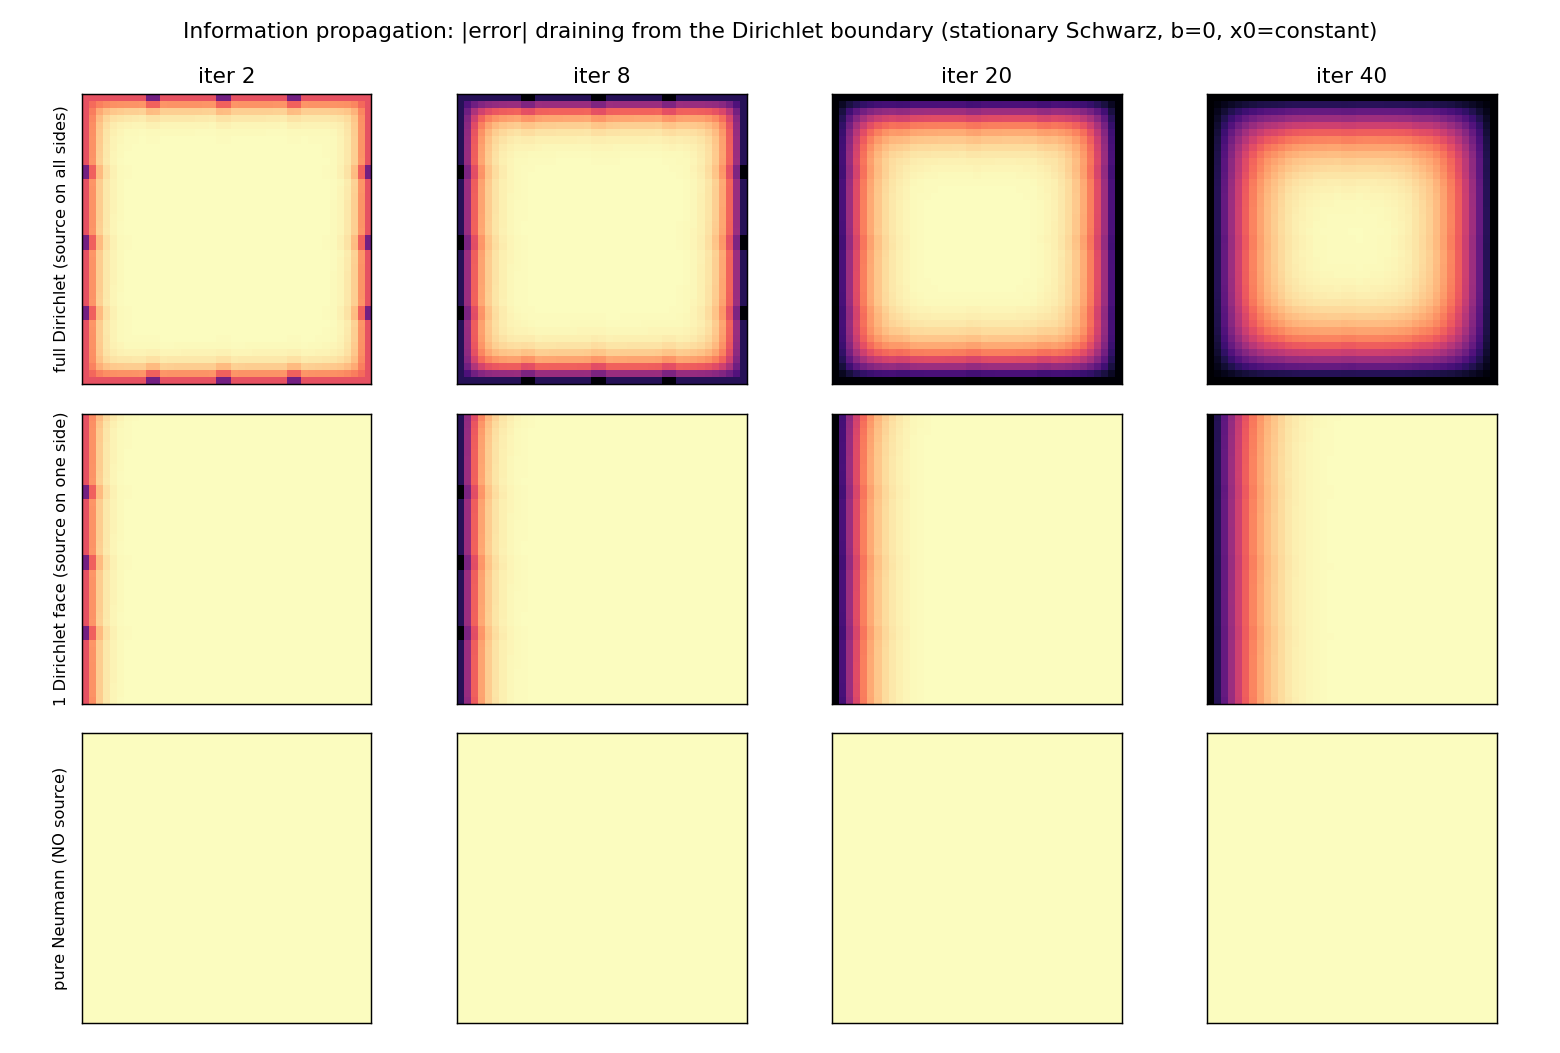
\includegraphics[width=\linewidth,height=0.62\textheight,keepaspectratio]{results/fig_info_prop_maps.png}
  \end{column}
  \begin{column}{0.34\linewidth}\footnotesize
   \spec{Setup:}{stationary (damped) Schwarz, $b{=}0$, $x_0{=}$constant (the global mode); plot $|$error$|$ per sweep.}
   \spec{Read it as:}{the Dirichlet boundary is the \emph{source} — error drains \emph{from} it inward, $\sim$one subdomain/sweep.}
   \spec{full Dirichlet:}{drains from all 4 sides $\Rightarrow$ fast, large $\lambda_{\min}$.}
   \spec{1 Dirichlet face:}{drains from one side only; far side lags $\Rightarrow$ small $\lambda_{\min}$.}
   \spec{pure Neumann:}{flat at every iter — \emph{no source}, the constant can't drain ($\lambda_{\min}{\to}0$, singular = Sys2).}
  \end{column}
  \end{columns}
  \concl{``Information propagation'' = the boundary value draining inward each sweep. \textbf{More Dirichlet boundary = more sources = faster fill = larger $\lambda_{\min}$.} Pure-Neumann has no source $\Rightarrow$ the global mode is undamped $\Rightarrow$ Sys2 is hardest — exactly what a coarse space must supply.}
\end{frame}

% ===================================================== PART II
{\setbeamercolor{background canvas}{bg=navy}\begin{frame}[plain]\centering\vfill
 {\color{amber}\Large\textbf{Part II}}\\[0.3em]{\color{white}\LARGE\bfseries Attribution}\\[0.4em]
 {\color{white!80!teal} which factor makes it hard, via which channel}\vfill\end{frame}}

\begin{frame}{Attribution: dimension $\to\lambda_{\max}$, boundary/shift $\to\lambda_{\min}$}{Part II}
  \begin{columns}[T]
  \begin{column}{0.42\linewidth}\footnotesize
   \spec{Studies:}{is it 3D, Dirichlet, Neumann, or shift that makes it hard?}
   \spec{Problem:}{$A=K+\sigma I$ ($\sigma$ large $\approx$ Sys1, $\sigma{\to}0\approx$ Sys2), FD grid.}
   \spec{BC axis:}{full / $k$-Dir faces / 1-Dir (mixed) / pure-Neumann $\sigma\in\{10,1,0.1\}$.}
   \spec{Size:}{2D $M{=}25$ (N=625), 3D $M{=}13$ (N=2197); S=4.}
   \spec{Params:}{overlap 0–3; ICC(0); ASM \& sASM.}
   \spec{Result:}{$\lambda_{\max}$=2D 4.30/3D 8.31 ($=\hat N$), FLAT over BC/$\sigma$; $\lambda_{\min}$ collapses $\sim$190$\times$(2D)/300$\times$(3D); $\kappa\propto1/\sigma$.}
  \end{column}
  \begin{column}{0.56\linewidth}\centering
   \rfig[1.0]{fig_attrib_channels_2d.png}\\
   {\scriptsize\color{muted}\textit{$\lambda_{\max}$ flat (over-count, set by dimension); $\lambda_{\min}$ collapses (info transfer, set by boundary/$\sigma$); iters track $\lambda_{\min}$.}}
  \end{column}
  \end{columns}
  \concl{No single culprit — \textbf{dimension sets $\lambda_{\max}$ (over-count $\hat N{=}2^d$), boundary/shift set $\lambda_{\min}$}; they are orthogonal and multiply. Sys2 ($\sigma{\to}0$, pure-Neumann, singular) = hardest. Overlap/sASM cannot touch $\lambda_{\min}$ $\Rightarrow$ need a coarse space.}
\end{frame}

% ===================================================== PART III
{\setbeamercolor{background canvas}{bg=navy}\begin{frame}[plain]\centering\vfill
 {\color{amber}\Large\textbf{Part III}}\\[0.3em]{\color{white}\LARGE\bfseries A non-GenEO coarse space}\\[0.4em]
 {\color{white!80!teal} shift-invariant spectral + known-coefficient modes}\vfill\end{frame}}

% ----- III.a shift-invariant -----
\begin{frame}{III.a Shift-invariant $(K,M)$ spectral coarse}{Part III $\cdot$ coarse}
  \begin{columns}[T]
  \begin{column}{0.42\linewidth}\footnotesize
   \spec{Studies:}{one coarse basis valid across the whole Sys1$\to$Sys2 ($\sigma$) range.}
   \spec{Problem:}{pure-Neumann $K$, $A=K+\sigma I$.}
   \spec{Size:}{2D $M{=}25$ (N=625), S=4, O=1.}
   \spec{Params:}{$\sigma\in\{10,1,0.1,0.01\}$; coarse modes $m\in\{1,4,8,16\}$; $V_0=$ low eigvecs of $K$, built ONCE.}
   \spec{Result:}{one-level $\kappa$ 53$\to$52000 as $\sigma{\to}$0; two-level $m{=}1$ (constant) caps $\kappa\approx54$ flat; $m{=}16\Rightarrow\kappa\approx5$.}
  \end{column}
  \begin{column}{0.56\linewidth}\centering
   \rfig[1.0]{fig_shiftinv.png}\\
   {\scriptsize\color{muted}\textit{$A_0=\Lambda_{\text{low}}+\sigma I$: same $V_0$ for all $\sigma$; $\lambda_0\approx0$ mode = constant = Sys2 nullspace.}}
  \end{column}
  \end{columns}
  \concl{One basis (built once from $K$) spans Sys1$\to$Sys2; the constant mode deflates the Sys2 singularity ($m{=}1$ already removes the $\sigma{\to}0$ blow-up).}
\end{frame}

% ----- III.b known-coefficient -----
\begin{frame}{III.b Known-coefficient A-harmonic modes (non-GenEO)}{Part III $\cdot$ coarse}
  \begin{columns}[T]
  \begin{column}{0.42\linewidth}\footnotesize
   \spec{Studies:}{handle high-contrast without GenEO eigenproblems.}
   \spec{Problem:}{$-\nabla\!\cdot(a\nabla u)=f$, mixed BC, FD.}
   \spec{Size:}{2D $M{=}25$ (N=625), S=4, O=1.}
   \spec{Params:}{coef $\in$\{const, layers, checker\}, $\rho{=}10^4$; constructions = global spectral / raw indicator / A-harmonic / hybrid.}
   \spec{Result:}{checker: A-harmonic 13 modes $\Rightarrow\kappa{=}646$ ($=$ global spectral $m{=}32$); hybrid (4 spec+coef) $30\times$ better than spectral-only at equal modes.}
  \end{column}
  \begin{column}{0.56\linewidth}\centering
   \rfig[1.0]{fig_coarse_coef.png}\\
   {\scriptsize\color{muted}\textit{A-harmonic known-coef modes reach the robustness floor with $\sim$half the modes of blind global spectral.}}
  \end{column}
  \end{columns}
  \concl{Build contrast modes from the \textbf{known} conductivity regions (cardiac fibers/$\sigma_i,\sigma_e$) instead of discovering them — same robustness, far fewer modes, no eigenproblems.}
\end{frame}

% ===================================================== PART IV
{\setbeamercolor{background canvas}{bg=navy}\begin{frame}[plain]\centering\vfill
 {\color{amber}\Large\textbf{Part IV}}\\[0.3em]{\color{white}\LARGE\bfseries Cross-system reuse}\\[0.4em]
 {\color{white!80!teal} Sys1$\to$Sys2 (same mesh), Sys3 (different mesh)}\vfill\end{frame}}

% ----- IV.a Sys1->Sys2 -----
\begin{frame}{IV.a Sys1$\to$Sys2: one build-once shared coarse}{Part IV $\cdot$ same mesh}
  \begin{columns}[T]
  \begin{column}{0.40\linewidth}\footnotesize
   \spec{Studies:}{reuse one hybrid coarse across Sys1$\to$Sys2 + a timestep sequence; beat Task-3's 1.6$\times$.}
   \spec{Problem/BC:}{shared heart mesh, $A=K+\sigma I$, pure-Neumann.}
   \spec{Size:}{2D $M{=}33$ (N=1089), S=4, O=1.}
   \spec{Params:}{$\sigma\in\{10^3..10^{-4}\}$; coef const/layers($\rho{=}10$); hybrid coarse (4 spectral + A-harmonic); sequence $T{=}12$ moving front at $\sigma{=}10^{-2}$.}
   \spec{Result:}{$\kappa$ flat over $\sigma$ (one-level $\propto1/\sigma\to4.7\mathrm{e}5$); sequence \textbf{919$\to$548 (1.68$\times$)}, +warm 541 (1.70$\times$).}
  \end{column}
  \begin{column}{0.58\linewidth}\centering
   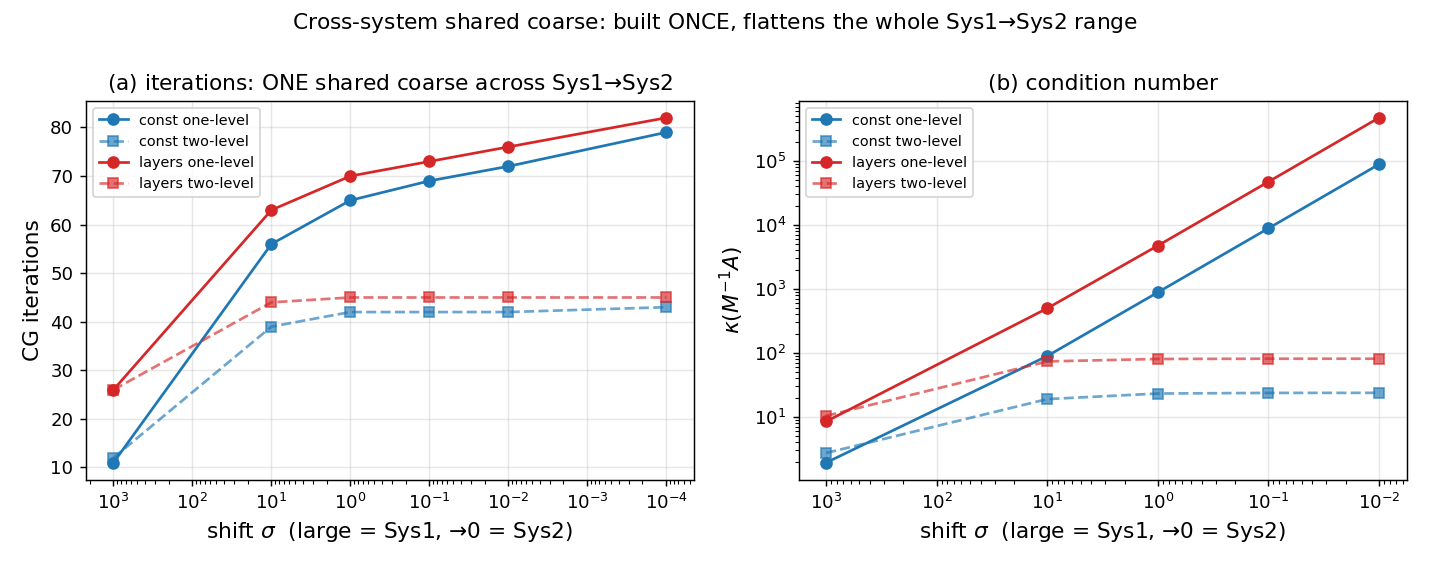
\includegraphics[width=\linewidth,height=0.34\textheight,keepaspectratio]{results/fig_xsys_sigma.png}\\[1pt]
   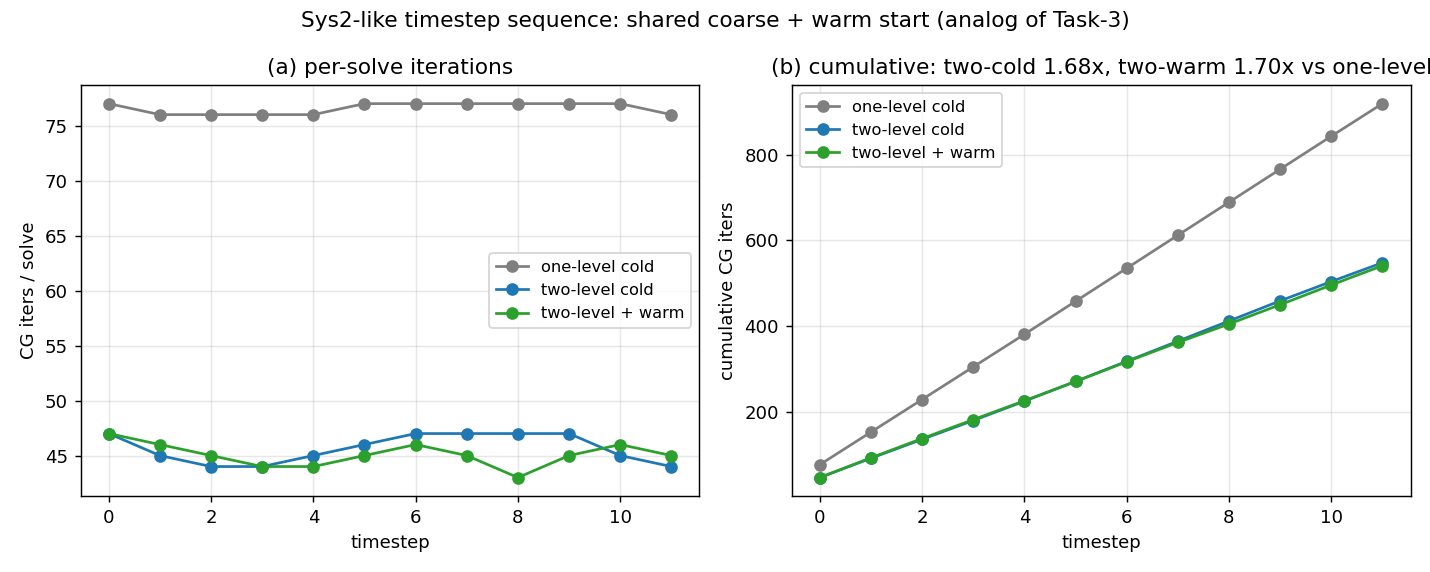
\includegraphics[width=\linewidth,height=0.30\textheight,keepaspectratio]{results/fig_xsys_sequence.png}
  \end{column}
  \end{columns}
  \concl{One coarse, built once, flattens the whole Sys1$\to$Sys2 range; \textbf{coarse is the main lever (1.68$\times$), warm-start marginal} — matches Task-3.}
\end{frame}

% ----- IV.b Sys3 -----
\begin{frame}{IV.b Sys3 (torso): cross-mesh interface scheme}{Part IV $\cdot$ different mesh}
  \begin{columns}[T]
  \begin{column}{0.42\linewidth}\footnotesize
   \spec{Studies:}{a different mesh, coupled only by the epicardial interface — reuse via per-mesh coarse + temporal coherence.}
   \spec{Problem/BC:}{torso Laplace; $x_0{=}0$ face = interface Dirichlet ($u_e$, moving front), rest Neumann; \emph{non-singular}.}
   \spec{Size:}{torso $M{=}41$ (N=1681) $\neq$ heart $M{=}33$; S=4, O=1.}
   \spec{Params:}{sequence $T{=}12$ moving-front interface data; per-mesh coarse $m{=}8$; one cold / two cold / two warm.}
   \spec{Result:}{\textbf{834$\to$406 (2.05$\times$)}, +warm 391 (2.13$\times$); eff-rank 8$\approx$Sys2's 7.}
  \end{column}
  \begin{column}{0.56\linewidth}\centering
   \rfig[1.0]{fig_sys3.png}\\
   {\scriptsize\color{muted}\textit{Per-mesh coarse is the lever (2.05$\times$); warm-start marginal — the moving front is moderate-rank on either mesh.}}
  \end{column}
  \end{columns}
  \concl{Cannot share the heart $V_0$, but the \emph{same construction} on the torso mesh gives 2.05$\times$. \textbf{Honest negative:} ``torso is much more warm-startable'' is \emph{not} supported (eff-rank 8$\approx$7).}
\end{frame}

% ===================================================== CONCLUSIONS
{\setbeamercolor{background canvas}{bg=navy}\setbeamercolor{normal text}{fg=white}
\begin{frame}[plain]\usebeamercolor[fg]{normal text}
  \vspace{0.4em}{\color{white}\Large\bfseries Unifying conclusions}\par\vspace{0.2em}{\color{teal}\rule{\linewidth}{1.4pt}}\vspace{0.5em}
  {\footnotesize\color{white}
  \begin{itemize}\setlength\itemsep{0.5em}
   \item[\textcolor{amber}{\textbf{1}}] \textbf{\textcolor{amber}{The anomaly is real and mechanistic:}} unscaled BASIC ASM + inexact ICC makes overlap raise $\lambda_{\max}{=}\omega\hat N$; sASM removes $\hat N$ and wins in 2D/3D (hurts only in 1D where $\omega{=}1$).
   \item[\textcolor{amber}{\textbf{2}}] \textbf{\textcolor{amber}{Two orthogonal channels:}} dimension sets $\lambda_{\max}$ ($\hat N{=}m_{\text{axis}}^d$); boundary \& shift set $\lambda_{\min}$. Sys2 (pure-Neumann, $\sigma{\to}0$) is hardest because $\lambda_{\min}{\to}0$ (singular).
   \item[\textcolor{amber}{\textbf{3}}] \textbf{\textcolor{amber}{A non-GenEO coarse fixes $\lambda_{\min}$:}} shift-invariant $(K,M)$ spectral modes (smooth + constant/nullspace, reused across $\sigma$) + known-coefficient A-harmonic modes (contrast, few modes, no eigenproblems).
   \item[\textcolor{amber}{\textbf{4}}] \textbf{\textcolor{amber}{Coarse is the cross-system lever:}} Sys1$\to$Sys2 (same mesh) 1.68$\times$, Sys3 (different mesh) 2.05$\times$; warm-start/POD marginal everywhere (moving front is moderate-rank) — reproducing Task-3 across all three systems.
  \end{itemize}}
\end{frame}}

% ===================================================== LIMITATIONS / NEXT
\begin{frame}{Limitations \& next steps}{appendix}
  \begin{columns}[T]
  \begin{column}{0.5\linewidth}\footnotesize
   \textcolor{teal}{\textbf{Limitations (honest)}}
   \begin{itemize}\setlength\itemsep{0.3em}
     \item Coarse-space results on a NumPy exact-spectrum proxy with scalar-contrast fields, not the real tensor anisotropy.
     \item Speedups (1.68$\times$, 2.05$\times$) are proxy values benchmarked against Task-3's real-pipeline 1.6$\times$.
     \item $\sigma{=}0$ exact singular handled by nullspace deflation (constant in $V_0$).
   \end{itemize}
  \end{column}
  \begin{column}{0.5\linewidth}\footnotesize
   \textcolor{teal}{\textbf{Next steps}}
   \begin{itemize}\setlength\itemsep{0.3em}
     \item Port the A-harmonic construction to the FEM fiber/conductivity tensor (cardiac $\sigma_i,\sigma_e$).
     \item Scale up in PETSc 3.24 on the real cardiac mesh; re-author \texttt{xsys\_precond.c}.
     \item Front-following interface enrichment for Sys3 (minor refinement per the data).
   \end{itemize}
  \end{column}
  \end{columns}
  \concl{Tooling: \texttt{asm\_spectral.py}, \texttt{schwarz\_fem.c}, \texttt{coarse\_proto.py}, \texttt{xsys\_proto.py}, \texttt{sys3\_proto.py}; all data \& figures on branch \texttt{influencing-factors-discussion}.}
\end{frame}

\end{document}
